\chapter{Quality at Glance}

\section{Introduction}
Access to multilingual datasets for NLP research has vastly improved over the past years. A variety of web-derived collections for hundreds of languages is available for anyone to download, such as ParaCrawl~\citep{espla-etal-2019-paracrawl, banon-etal-2020-paracrawl}, WikiMatrix~\citep{schwenk-etal-2021-wikimatrix} CCAligned~\citep{el-kishky-etal-2020-ccaligned}, \mbox{OSCAR}~\citep{ortiz-suarez-etal-2019-asynchronous, ortiz-suarez-etal-2020-monolingual}, and several others.
%though ma \citep{joshi-etal-2020-state}.
These have in turn enabled a variety of highly multilingual models, like mT5 \citep{xue-etal-2021-mt5}, M2M\nobreakdash-100 \citep{fan-etal-2020-beyond}, M4 \citep{arivazhagan-etal-2019-massively}.
% Recent approaches that employ large-scale multilingual systems have shown potential for some generalization across typologically different languages \cite{pires-etal-2019-multilingual,papadimitriou-etal-2021-deep}. .

Curating such datasets relies on the websites giving clues about the language of their contents (e.g. a language identifier in the URL) and on automatic language classification (LangID).
%and filtering tools, and a range of evaluation sets and metrics to compile high-quality datasets. 
It is commonly known that these automatically crawled and filtered datasets tend to have overall lower quality than hand-curated collections~\citep{koehn-etal-2020-findings}, but their quality is rarely measured directly, and is rather judged through the improvements they bring to downstream applications~\citep{schwenk-etal-2021-wikimatrix}.

Building NLP technologies with automatically crawled datasets is promising. This is especially true for low-resource languages, because data scarcity is one of the major bottlenecks for deep learning approaches.
However, there is a problem: There exists very little research on evaluating both data collections and automatic crawling and filtering tools for low-resource languages.
As a result, although many low-resource languages are covered by the latest multilingual crawl data releases, their quality and thus usability is unknown. %Inferring the quality from higher-resource, well-evaluated and studied subsets of the same crawls would be rather naive, since errors can accumulate easily in the pipeline of multilingual web mining.

%ideas for start:
%\begin{itemize}
%    \item ``How good is my data?'' -- data quality becomes more and more of a concern with scaling up: giant models feeding on giant collections of (multimodal) data collections, facilitated by the easy access to data on the web. 
%    \item work we could cite:
%    \item On paper/in theory/in principle/according to raw data statistics, the situation for low-resource languages should have improved over the past year, with large multilingual data collections being released publicly. (insert example) The prospects for building NLP technologies on the base of these collections seem promising, since data sparsity is one of the bottlenecks for the application of current deep learning approaches. However, ...
%\end{itemize}
%While companies frequently use in-house curated data sets, these data sets are used frequently for academic research and publications, so it was important to understand them better.
To shed light on the quality of data crawls for the lowest resource languages, we perform a manual data audit for 230 per-language subsets of five major crawled multilingual datasets: CCAligned~\citep{el-kishky-etal-2020-ccaligned}, ParaCrawl~\citep{espla-etal-2019-paracrawl,banon-etal-2020-paracrawl}, WikiMatrix~\citep{schwenk-etal-2021-wikimatrix}, OSCAR~\citep{ortiz-suarez-etal-2019-asynchronous, ortiz-suarez-etal-2020-monolingual} and mC4~\citep{xue-etal-2021-mt5}. We propose solutions for effective, low-effort data auditing (section~\ref{sec:audit}), including an error taxonomy. Our quantitative analysis reveals surprisingly low amounts of valid in-language data, and identifies systematic issues across datasets and languages. In addition, we find that a large number of datasets is labeled with nontransparent or incorrect language codes (section~\ref{sec:codes}). This leads us to reflect on the potential harm of low-quality data releases for low-resource languages (section~\ref{sec:risk}), and provide a set of recommendations for future multilingual data releases (section~\ref{sec:recommendation}).

% The contributions of this paper are as follow:
% \begin{itemize}
%   \item We provide quantitative quality evaluations for 124 languages in five public datasets
%   \item We demonstrate that native-speaker expertise is not necessary to XXX 
%     \item the comparison across languages and corpora lets us identify the main pain points for future work 
%       \item reflection on the harm of low-quality data releases for low-resource languages (Section~\ref{sec:risk})
% \end{itemize}

\begin{table*}[th]
    \centering
    \resizebox{\textwidth}{!}{%
        \begin{tabular}{lccccc}
            \toprule
                            & \multicolumn{3}{c}{\textbf{Parallel}} & \multicolumn{2}{c}{\textbf{Monolingual}}                                                       \\
            \cmidrule(lr){2-4} \cmidrule(lr){5-6}
                            & \textbf{CCAligned}                    & \textbf{ParaCrawl v7.1}                  & \textbf{WikiMatrix} & \textbf{OSCAR} & \textbf{mC4} \\
            \midrule
            \#languages     & 137                                   & 41                                       & 85                  & 166            & 101          \\
            Source          & CC 2013--2020                         & selected websites                        & Wikipedia           & CC 11/2018     & CC all       \\
            Filtering level & document                              & sentence                                 & sentence            & document       & document     \\
            Langid          & FastText                              & CLD2                                     & FastText            & FastText       & CLD3         \\
            Alignment       & LASER                                 & Vec/Hun/BLEU-Align                       & LASER               & -              & -            \\
            Evaluation      & TED-6                                 & WMT-5                                    & TED-45              & POS/DEP-5      & XTREME       \\
            \bottomrule
        \end{tabular}%
    }
    \caption{Comparison of parallel and monolingual corpora extracted from web documents, including their downstream evaluation tasks. All parallel corpora are evaluated through machine translation evaluation with BLEU. TED-6: \texttt{da}, \texttt{cr}, \texttt{sl}, \texttt{sk}, \texttt{lt}, \texttt{et}; TED-45: 45-language subset of ~\citep{qi-etal-2018-pre}; WMT-5: \texttt{cs}, \texttt{de}, \texttt{fi}, \texttt{lv}, \texttt{ro}. POS/DEP-5: part-of-speech labeling and dependency parsing for \texttt{bg}, \texttt{ca}, \texttt{da}, \texttt{fi}, \texttt{id}.}
    \label{tab:corpora}
\end{table*}
% CC: CommonCrawl; TED-6: da, cr, sl, sk, lt, et; TED-50: TODO cite Qi et al. 2018; WMT-5: cs, de, fi, lv, ro.
%fastText: 176 languages, Wikipedia & Tatoeba

\section{Related Work}\label{sec:related}

Corpora collected by web crawlers are known to be noisy~\citep{junczys-dowmunt-2019-microsoft}. In highly multilingual settings, past work found that web-crawls of lower-resource languages have serious issues, especially with segment-level LangID~\citep{caswell-etal-2020-language}.
%Repeated studies have shown that 
Cleaning and filtering web-crawls can boost general language modeling~\citep{gao-etal-2020-the,brown-etal-2020-language,raffel-etal-2020-exploring} and downstream task performance~\citep{moore-lewis-2010-intelligent,xu-koehn-2017-zipporah,khayrallah-koehn-2018-impact,brown-etal-2020-language}.

% zaricna2015word
As the scale of ML research grows, it becomes increasingly difficult to validate automatically collected and curated datasets \citep{biderman-etal-2020-pitfalls,birhane-etal-2021-large,bender-etal-2021-on}.
%Data Quality Considerations for Big Data and Machine Learning: Going Beyond Data Cleaning and Transformations \citep{gudivada2017data}
Several works have focused on advancing methodologies and best practices to address these challenges. \citet{bender-friedman-2018-data} introduced data statements, a documentary framework for NLP datasets that seeks to provide a universal minimum bar for dataset description. Similar work has focused on
% been done on systematizing documentation in other areas in data science and machine learning, including work focusing on 
online news \citep{kevin-etal-2018-information}, data ethics \citep{sun-etal-2019-mithralabel}, and data exploration \citep{holland-etal-2018-the}, as well as generalist work such as \citep{gebru-etal-2018-datasheets}. There is a large literature on filtering text data for various NLP tasks, e.g. \cite{axelrod-etal-2011-domain,moore-lewis-2010-intelligent,wang-etal-2018-denoising,kamholz-etal-2014-panlex,junczys-dowmunt-2018-dual,caswell-etal-2020-language}.

Closest to our work is the analysis of a highly multilingual (non-publicly available) web-crawl and LangID related quality issues by \citet{caswell-etal-2020-language}.
%, performing a highly multilingual web-crawl and then systematically analyzing the LangID related quality issues. 
%However, though 
They perform a brief analysis of the quality of OSCAR
%, but omit analyses of any other public datasets, 
with the focus only on the presence of in-language content.

% Previous work also focused on automatic methods to improve data quality for both monolingual and parallel corpora.  proposes a method for filtering noisy parallel data based on cross-entropy scores of two inverse translation models which shows significant improvement over baselines models.  demonstrate that the language identification models for low-resource languages are almost unusable despite the belief that the task is ``solved". Authors propose two filtering techniques to alleviate common problems these models fall prey to. TODO: Jim: Just wrote this out fully as a reference. Might need to shorten it later.

% Diversity
% The availability of data resources has shaped research in NLP; most systems are trained and evaluated on a few dominant language families. On the other hand, resource-scarce languages have only recently started to receive attention with focused communities working on these languages \citep{joshi-etal-2020-state}. Recent approaches that employ large-scale multilingual systems have shown potential for some generalization across typologically different languages, relying only on an unlabeled monolingual datasets \cite{pires-etal-2019-multilingual,papadimitriou-etal-2021-deep}. 
% 

% TODO: Summarize the following related works into coherent paragraphs.
% \paragraph{Corpus cleaning}
% \begin{itemize}
% % \item Dual Conditional Cross-Entropy Filtering of Noisy Parallel Corpora \citep{junczys-dowmunt-2018-dual} (covered)
% % \item Language ID in the Wild: Unexpected Challenges on the Path to a Thousand-Language Web Text Corpus. \citep{caswell-etal-2020-language} (covered)
% \item Garbage in Garbage Out \citet{geiger2020garbage} (this wasn't really about corpus cleaning. not sure how to include it)
% \end{itemize}

% \paragraph{Reports about data noise}
% \begin{itemize}
%     \item Language ID in the Wild: Unexpected Challenges on the Path to a Thousand-Language Web Text Corpus  \citep{}
%     \item Comparing parallel corpora and evaluating their quality \citep{kaalep2007comparing} (this is not included yet but the scope if smaller than others)
% \end{itemize}

%NLP data quality evaluation

% \paragraph{Diversity / low-resource language representation in NLP}
% \begin{itemize}
%     % \item The State and Fate of Linguistic Diversity and Inclusion in the NLP World \citep{joshi-etal-2020-state}
%     % \item How Multilingual is Multilingual BERT? \citep{pires-etal-2019-multilingual} 
%     \item Findings of the WMT 2019 Shared Task on Parallel Corpus Filtering for Low-Resource Conditions \citep{koehn-etal-2019-findings}
% \end{itemize}

% \paragraph{Nutrition Labels \& datasheets}
% \begin{itemize}
%     \item Datasheets for Datasets 
%     \item The Dataset Nutrition Label: A Framework To Drive Higher Data Quality Standards \cite{holland-etal-2018-the}
% \end{itemize}


\section{Multilingual Corpora}\label{sec:crawls}
Table \ref{tab:corpora} provides an overview of the corpora of interest in this work. We selected the corpora for their multilinguality and the inclusion of understudied languages in NLP. With the exception of WikiMatrix and Paracrawl, all corpora are derived from CommonCrawl (CC).\footnote{\url{http://commoncrawl.org/}} %s, and distinguish themselves by the choice of filtering methods, LangID and automatic alignment technology.
%LangID is crucial to corpus creation, since any issues within might propagate, e.g. bias recognizing document types similar to what it was trained on, or errors in language identifiers.\footnote{\url{https://github.com/facebookresearch/fastText/issues/482}}



%TODO briefly describe recipe for web-mining data like in https://arxiv.org/pdf/2010.14571.pdf in Appendix K 
%Describe pipeline to get to a crawled corpus for a language or at least which components play a role, so that we can later refer to them and partially explain the type of garbage that ends up there and point out the bottlenecks (lang id!!!!) for anyone out there looking for research projects. (Note: https://arxiv.org/pdf/2010.14571.pdf in Appendix K gives a recipe for web-mining data)

%TODO: briefly mention what each dataset has been used for

\paragraph{CCAligned~\citep{el-kishky-etal-2020-ccaligned}}is a %119-language\footnote{119 of originally 137 available for download (02/2021)}
%Although 137 language pairs are reported in ~\citet{el-kishky-etal-2020-ccaligned}, only 119 sentence-level corpora were available to download on \url{statmt.org} as of February 2021.}
parallel dataset built off 68 CC snapshots. Documents are aligned if they are in the same language according to FastText LangID~\citep{joulin-etal-2016-fasttext,joulin-etal-2017-bag}, and have the same URL but for a differing language code. These alignments are refined with cross-lingual LASER embeddings \citep{artetxe-schwenk-2019-massively}. For sentence-level data, they split on newlines and align with LASER, but perform no further filtering.
Human annotators evaluated the quality of document alignments for six languages (\texttt{de}, \texttt{zh}, \texttt{ar}, \texttt{ro}, \texttt{et}, \texttt{my}) selected for their different scripts and amount of retrieved documents, reporting precision of over 90\%.
% Latin, Chinese, Arabic, Burmese script
The quality of the extracted parallel sentences was evaluated in a machine translation (MT) task on six European (\texttt{da}, \texttt{cr}, \texttt{sl}, \texttt{sk}, \texttt{lt}, \texttt{et}) languages of the TED corpus~\citep{qi-etal-2018-pre}, where it compared favorably to systems built on crawled sentences from WikiMatrix and ParaCrawl v6. %, yielding BLEU scores in a range between 15 and 38.  

\paragraph{Multilingual C4 (mC4)~\citep{xue-etal-2021-mt5}} is a document-level dataset used for training the mT5 language model. It consists of monolingual text in 101 languages and is generated from 71 CC snapshots. It filters out pages that contain less than three lines of at least 200 characters and pages that contain bad words~\citep{emerick-2018-list}. Since this is a document-level dataset, we split it by sentence and deduplicate it before rating. For language identification, it uses CLD3~\citep{botha-etal-2017-natural}, a small feed-forward neural network that was trained to detect 107 languages.
% \footnote{\url{https://github.com/LDNOOBW/}}
% \footnote{\url{https://github.com/google/cld3/}}
The mT5 language model pre-trained on mC4
%\footnote{Upsampling lower-resource languages.} 
is evaluated on 6 tasks of the XTREME benchmark~\citep{hu-etal-2020-xtreme} covering a variety of languages and outperforms other multilingual pre-trained language models such as mBERT~\citep{devlin-etal-2019-bert} and XLM\nobreakdash-R~\citep{conneau-etal-2020-unsupervised}.%\footnote{mBERT is trained on Wikipedia, {XML\nobreakdash-R} on CommonCrawl.} 

\paragraph{OSCAR~\citep{ortiz-suarez-etal-2019-asynchronous, ortiz-suarez-etal-2020-monolingual}}is a set of monolingual corpora extracted from CC snapshots, specifically from the plain text \emph{WET} format distributed by CC which removes all the HTML tags and converts the text formatting to UTF-8. It is deduplicated and follows the same approach as~\citet{grave-etal-2018-learning} by using FastText LangID
%~\citep{joulin-etal-2016-fasttext, joulin-etal-2017-bag} 
on a line-level.
%No other filtering was applied.
% \footnote{\url{https://fasttext.cc/docs/en/language-identification.html}
For five languages (\texttt{bg}, \texttt{ca}, \texttt{da}, \texttt{fi}, \texttt{id}) OSCAR corpora were used to train ELMo~\citep{peters-etal-2018-deep} embeddings for POS tagging and dependency parsing, outperforming those trained on Wikipedia~\citep{ortiz-suarez-etal-2020-monolingual}. % -sourced embeddings


\paragraph{ParaCrawl v7.1} is a parallel dataset with 41 language pairs primarily aligned with English (39 out of 41) and mined using the parallel-data-crawling tool Bitextor \citep{espla-etal-2019-paracrawl,banon-etal-2020-paracrawl} which includes downloading documents, preprocessing and normalization, aligning documents and segments, and filtering noisy data via Bicleaner.
% \footnote{\url{https://github.com/bitextor/bicleaner}}
ParaCrawl focuses on European languages, but also includes 9 lower-resource, non-European language pairs in v7.1.
% TODO: https://www.aclweb.org/anthology/2020.eamt-1.31.pdf \citep{ramirez-sanchez-etal-2020-bifixer}
Sentence alignment and sentence pair filtering choices were optimized for five languages (\texttt{mt}, \texttt{et}, \texttt{hu}, \texttt{cs}, \texttt{de}) by training and evaluating MT models on the resulting parallel sentences. An earlier version, ParaCrawl v5, was shown to improve translation quality on WMT benchmarks for~\texttt{cs}, \texttt{de}, \texttt{fi}, \texttt{lv}, \texttt{ro}.


\paragraph{WikiMatrix~\citep{schwenk-etal-2021-wikimatrix}}is a public dataset containing 135M parallel sentences in 1620 language pairs (85 languages) mined from Wikipedia. Out of the 135M parallel sentences, 34M are aligned with English.
%which relies on first learning multilingual sentence embeddings, and then applying the cosine distance metric to determine whether two sentences are close enough to be considered translations of each other.
The text is extracted from Wikipedia pages, split into sentences, and duplicate sentences are removed. FastText LangID is used before identifying bitext with LASER's distance-based mining approach.
The margin threshold is optimized by training and evaluating downstream MT models on four WMT benchmarks (\texttt{de-en}, \texttt{de-fr}, \texttt{cs-de}, \texttt{cs-fr}). The final dataset is evaluated through TED translation models between 45 languages, with highest quality for translations between English and e.g. \texttt{pt}, \texttt{es}, \texttt{da}, and lowest for \texttt{sr}, \texttt{ja}, \texttt{mr}, \texttt{zh\_TW}.
%In the audit 
We focus on language pairs with English on one side.
% https://github.com/facebookresearch/LASER/blob/master/tasks/WikiMatrix/WikiMatrix-bleu.pdf
%TODO used for example in https://arxiv.org/abs/2010.11125
%TODO used in https://www.aclweb.org/anthology/2020.emnlp-main.121.pdf 

%\paragraph{FastText LangID}
%The FastText~\citep{grave-etal-2018-learning} language classifier was trained on Wikipedia, Tatoeba, SETimes,\footnote{\url{https://fasttext.cc/docs/en/language-identification.html}} so any issues within these collections might propagate, and there might be a bias recognizing similar document types, e.g. lexicon entries, in CC. 176 languages



\section{Auditing Data Quality}\label{sec:audit}
None of the above datasets has been evaluated for quality on the sentence level (exception: several languages in ParaCrawl v3), and downstream evaluations are centered around a small fraction of higher-resource languages. This is insufficient for drawing conclusions about the quality of individual or aligned sentences, and about the entirety of languages. %but only on document/URL level and a small selection of downstream tasks. 
%: Samples of URLs or retrieved documents were evaluated for their accuracy, and derived Machine Translation (MT) and NLP systems are shown to perform well for a subset of language pairs. 
%This does not guarantee that individual or aligned sentences extracted from those documents or URLs are of high quality, nor is the subset of languages sufficient to guarantee for the data quality of the whole corpus. %(TODO stats).
% Additionally: publication bias: negative results might not have been published (are harder to publish)
%excuse: no speaker available, reality: speaker not necessarily needed
To close this gap, we conduct a data quality audit that focuses on the lowest-resource and most under-evaluated languages, but also covers mid- and high-resource languages for comparison. %; and (2) aims at width rather than depth in order to draw comparisons across datasets and languages.


\begin{table*}[th]
    \small
    \centering
    \begin{tabular}{|ll|}
        \hline
        \hline
        \multicolumn{2}{|c|}{\textbf{Correct Codes}}                                                                                \\
        \hline
        \multicolumn{2}{|l|}{\textbf{\texttt{CC}:} \textit{Correct translation, natural sentence}}                                  \\
        \hdashline
        \texttt{en} The Constitution of South Africa            & \texttt{nso} Molaotheo wa Rephabliki ya Afrika Borwa              \\
        \texttt{en} Transforming your swimming pool into a pond & \texttt{de} Umbau Ihres Swimmingpools zum Teich                   \\
        \hline
        \multicolumn{2}{|l|}{\textbf{\texttt{CB}:} \textit{Correct translation, Boilerplate or low quality}}                        \\
        \hdashline
        \texttt{en} Reference number: 13634                     & \texttt{ln} Motango ya référence: 13634                           \\
        \texttt{en} Latest Smell Stop Articles                  & \texttt{fil} Pinakabagong mga Artikulo Smell Stop                 \\
        %  \texttt{en} Weight (Male): 8,6 - 13,5 kg & \texttt{ts} Ntiko (Xinuna): 8, 6 - 13, 5 kg \\
        \hline
        \multicolumn{2}{|l|}{\textbf{\texttt{CS}:} \textit{Correct translation, Short}}                                             \\
        \hdashline
        \texttt{en} movies, dad                                 & \texttt{it} cinema, pap\`{a}                                      \\
        \texttt{en} Halloween - without me                      & \texttt{ay} Hallowen – janiw nayampejj                            \\
        \hline
        \hline
        \multicolumn{2}{|c|}{\textbf{Error Codes}}                                                                                  \\
        \hline
        \multicolumn{2}{|l|}{\textbf{X:} \textit{Incorrect translation, but both correct languages}}                                \\
        \hdashline
        \texttt{en} A map of the arrondissements of Paris       & \texttt{kg} Paris kele mbanza ya kimfumu ya Fwalansa.             \\
        \texttt{en} Ask a question                              & \texttt{tr} Soru sor Kullanıma g{\"o}re se\c{c}im                 \\
        \hline
        \multicolumn{2}{|l|}{\textbf{\texttt{WL}:} \textit{Source OR target wrong language, but both still linguistic content}}     \\
        \hdashline
        \texttt{en} The ISO3 language code is zho               & \texttt{zza} T{\' a}im eadra bracach mar bhionns na frogannaidhe. \\
        %  \texttt{en} sicilianu: Johannesburg & \texttt{ve} Tshivenda: Johannesburg \\
        \texttt{en} Der Werwolf — sprach der gute Mann,         &
        \texttt{de} des Weswolfs, Genitiv sodann,                                                                                   \\
        \hline
        \multicolumn{2}{|l|}{\textbf{NL:} \textit{Not a language: at least one of source and target are not linguistic content}}    \\
        \hdashline
        \texttt{en} EntryScan 4 \_                              & \texttt{tn} TSA PM704 \_                                          \\
        \texttt{en} organic peanut butter                       & \texttt{ckb} \ucr \ucr \ucr \ucr \ucr \ucr \ucr                   \\
        \bottomrule
    \end{tabular}
    \caption{Annotation codes for parallel data with sentence pair examples. The language code before each sentence indicates the language it is supposed to be in.}
    \label{tab:examples}
\end{table*}

\subsection{Auditing Process}

\paragraph{Participants} We recruited 51 volunteers from the NLP community, covering about 70 languages with proficient language skills.
%\footnote{This surprisingly high number comes in part because there are many closely related languages, e.g. one person may be proficient enough to rate many different Slavic or Turkic languages even if only one is their native language.} 
To verify our hypothesis that those annotations can largely done by non-native speakers, we repeat a set of language expert annotations by a non-expert, and measure the accuracy of the non-expert.

\paragraph{Sample selection} For each language in each dataset, we took a random sample of 100 lines, which may be anywhere from single words to short paragraphs depending on segmentation.% (see last columns in tables in appendix~\ref{app:stats}).
%While we will speak of ``sentences'', these might be single words or paragraphs according depending on the segmentation of the datasets in their published form.%\footnote{For the monolingual document-level dataset MC4, we split on sentences before evaluating.} 
We manually annotated them according to the error taxonomy described below. For WikiMatrix and CCAligned, we selected those languages that are paired with English, and for ParaCrawl, we also included those paired with Spanish (``total'' counts in table~\ref{tab:results}).
We did not annotate all languages, but focused on the ones with the least number of sentences in each dataset (at least the smallest 10) and languages for which we found proficient speakers.
% Since we annotate the same maximum number of sentences\footnote{Some languages had fewer than 100 sentences.} across all chosen languages regardless of their total number of sentences, the annotated samples are not an unbiased sample from the whole dataset. 
%For the interpretation of our results this means that if our set of samples is e.g. 30\% correct, it does not mean that 30\% of the overall dataset is correct. 
%Prior evaluations have been biased towards the higher-resource and more widely studied languages in NLP that have existing benchmarks~\citep{joshi-etal-2020-state}, so our evaluation aims to do the opposite.


\paragraph{Non-expert labeling strategies}
Although many of the volunteers were familiar with the languages in question or spoke related languages, in cases where no speaker of a relevant language could be found, volunteers used dictionaries and internet search to form educated guesses. We discuss this deeper in  appendix~\ref{app:strategies} to highlight how much of this low-resource focused evaluation can actually be done by non-proficient speakers with relatively low effort.
%, and therefore should not constitute as much as a bottleneck as often depicted. % TODO and note high IAA between speakers and nonspeakers....
%TODO report remaining unknowns and potential mislabelings, e.g. confusion with closely related languages e.g. Nynorsk and Bokm\r{a}l.
In general, we aim to find an upper bound on quality, so we encouraged annotators to be forgiving of translation mistakes when the overall meaning of the sentence or large parts thereof are conveyed, or when most of the sentence is in the correct language.

% \paragraph{Effort} The individual effort was dependent on the quality and complexity of the data as well as the annotator's knowledge of the language(s), e.g., it took from less than two minutes for an English native speaker to pass through 100 well-formed English sentences (and it was similarly fast to annotate languages with 0\% in-language sentences), to two hours of ``detective work'' for well-formed content in languages where the annotator had no familiarity.

% for Celtic languages to triangulate meaning parallelism to English through a third language.

%For this work we only rate sentence-level datasets. For the monolingual document-level dataset MC4, we split on sentences before evaluating.

%TODO which percentage of audits were done with native speaker knowledge?

%TODO plot: size of corpus vs percentage of noise/clean data

%TODO plot: number of speakers vs percentage of noise/clean data

%\subsection{Taxonomy}
% Describe it and explain why (move it to the appendix later if it takes too much space)
\paragraph{Taxonomy}
In order to quantify errors, we developed a simple error taxonomy. Sentences and sentence pairs were annotated according to a simple rubric with error classes of Incorrect Translation (\texttt{X}, excluded for monolingual data), Wrong Language (\texttt{WL}), and Non-Linguistic Content (\texttt{NL}). Of correct sentences (\texttt{C}), we further mark single words or phrases (\texttt{CS}) and boilerplate contents (\texttt{CB}). The appendix contains the detailed instructions, and table \ref{tab:examples} provides examples for parallel data.
%For monolingual data, we exclude the \texttt{X} class. 
In addition, we asked annotators to flag offensive or pornographic content.

\begin{table*}[th]
    \centering\small
    % \resizebox{\textwidth}{!}{%
    \begin{tabular}{llccccc}
        \toprule
                                                                  &                             & \multicolumn{3}{c}{\textbf{Parallel}} & \multicolumn{2}{c}{\textbf{Monolingual}}                                                       \\
        \cmidrule(lr){3-5} \cmidrule(lr){6-7}
                                                                  &                             & \textbf{CCAligned}                    & \textbf{ParaCrawl v7.1}                  & \textbf{WikiMatrix} & \textbf{OSCAR} & \textbf{mC4} \\
        \midrule
        \multicolumn{2}{l}{\#langs audited / total}               & 65 / 119                    & 21 / 38                               & 20 / 78                                  & 51 / 166            & 48 / 108                      \\
        \multicolumn{2}{l}{\%langs audited}                       & 54.62\%                     & 55.26\%                               & 25.64\%                                  & 30.72\%             & 44.44\%                       \\
        \multicolumn{2}{l}{\#sents audited / total}               & 8037 / 907M                 & 2214 / 521M                           & 1997 / 95M                               & 3517 / 8.4B         & 5314 / 8.5B                   \\
        \multicolumn{2}{l}{\%sents audited}                       & 0.00089\%                   & 0.00043\%                             & 0.00211\%                                & 0.00004\%           & 0.00006\%                     \\
        \midrule
        \multirow{6}{*}{\rotatebox[origin=c]{90}{\textbf{macro}}} &
        \texttt{C}                                                & 29.25\%                     & 76.14\%                               & 23.74\%                                  & 87.21\%             & 72.40\%                       \\
                                                                  & \texttt{X}                  & 29.46\%                               & 19.17\%                                  & 68.18\%             & -              & -            \\
                                                                  & \texttt{WL}                 & 9.44\%                                & 3.43\%                                   & 6.08\%              & 6.26\%         & 15.98\%      \\
                                                                  & \texttt{NL}                 & 31.42\%                               & 1.13\%                                   & 1.60\%              & 6.54\%         & 11.40\%      \\
                                                                  & offensive                   & 0.01\%                                & 0.00\%                                   & 0.00\%              & 0.14\%         & 0.06\%       \\
                                                                  & porn                        & 5.30\%                                & 0.63\%                                   & 0.00\%              & 0.48\%         & 0.36\%       \\
        \midrule
        \multirow{6}{*}{\rotatebox[origin=c]{90}{\textbf{micro}}} &
        \texttt{C}                                                & 53.52\%                     & 83.00\%                               & 50.58\%                                  & 98.72\%             & 92.66\%                       \\
                                                                  & \texttt{X}                  & 32.25\%                               & 15.27\%                                  & 47.10\%             & -              & -            \\
                                                                  & \texttt{WL}                 & 3.60\%                                & 1.04\%                                   & 1.35\%              & 0.52\%         & 2.33\%       \\
                                                                  & \texttt{NL}                 & 10.53\%                               & 0.69\%                                   & 0.94\%              & 0.75\%         & 5.01\%       \\
                                                                  & offensive                   & 0.00\%                                & 0.00\%                                   & 0.00\%              & 0.18\%         & 0.03\%       \\
                                                                  & porn                        & 2.86\%                                & 0.33\%                                   & 0.00\%              & 1.63\%         & 0.08\%       \\
        \midrule
                                                                  & \#langs =0\% \texttt{C}     & 7                                     & 0                                        & 1                   & 7              & 0            \\
        %& \#langs $<$5\% \texttt{C} & 14 & 0 & 2 & 7  & 0 \\
        %& \#langs $<$20\% \texttt{C} & 27 & 0 & 10 & 7 & 4 \\
                                                                  & \#langs $<$50\% \texttt{C}  & 44                                    & 4                                        & 19                  & 11             & 9            \\
                                                                  & \#langs $>$50\% \texttt{NL} & 13                                    & 0                                        & 0                   & 7              & 1            \\
                                                                  & \#langs $>$50\% \texttt{WL} & 1                                     & 0                                        & 0                   & 3              & 4            \\
        \bottomrule
    \end{tabular}%
    %  }
    \caption{Averages of sentence-level annotations across datasets and selected languages. Macro-avg: Each language is weighted equally in the aggregation, regardless of its size. Micro-avg: Each label is weighted by the fraction of sentences for that language in the overall annotated corpus, i.e., the annotations for higher-represented languages are upweighted, and annotations for lower-represented languages are downweighted. The bottom rows contain the number of languages that have 0\% sentences labeled \texttt{C} etc. }
    \label{tab:results}
\end{table*}

\subsection{Human Audit Results}\label{sec:audit-res}



\paragraph{Interpretation of Results}
For each language, we compute the percentage of each label within the 100 audited sentences.
Then, we either aggregate the labels across languages with equal weights (macro-average), or weight them according to their presence in the overall dataset (micro-average).
Note that the number of languages, the numbers of sentences per language and the choice of languages differ across datasets, both in the original release and in the selection for our audit, so the comparison of numbers across datasets has to be taken with a grain of salt. Our audit captures a decent ratio of languages (25--55\%, 2nd row in table~\ref{tab:results}), but only a tiny fraction of the overall number of sentences (0.00004--0.002\%). Appendix~\ref{app:stats}
contains the detailed audit results for each language and dataset. When we speak of ``low-'' and ``high''-resource languages, we mean languages with smaller or larger representation in the datasets at hand. When reporting language-specific results we use the original language identifiers of the datasets.

% \paragraph{What are the quality judgements on audited samples?} 
\paragraph{Which datasets have quality issues?}
%A summary of the results of the audit is given in Tables~\ref{tab:macro_results} and~\ref{tab:micro_results}.
The macro-averaged results show that the ratio of correct samples (``\texttt{C}'') ranges from 24\% to 87\%, with a large variance across the five audited datasets.
% Note that mC4 and OSCAR are monolingual datasets, so they do not require a correct alignment to another language to be labeled as correct.
Particularly severe problems were found in CCAligned and WikiMatrix, with 44 of the 65 languages that we audited for CCAligned containing under 50\% correct sentences, and 19 of the 20 in WikiMatrix. In total, 15 of the 205 language specific samples (7.3\%) contained not a single correct sentence.
For the parallel datasets we are also interested in the quantity of misaligned/mistranslated sentences (\texttt{X}). For WikiMatrix, two-thirds of the audited samples were on average misaligned. We noticed that sentences were often similar in structure, but described different facts (see table~\ref{tab:not_actually_parallel}).

While Table~\ref{tab:results} gives means and numbers of corpora passing certain thresholds, Figure~\ref{fig:ratio_c} illustrates per-corpus correctness more completely, showing for each dataset what percent of audited corpora are under each possible threshold of correctness.

\paragraph{Why haven't these problems been reported before?}
The findings above are averaged on a per-language basis (i.e. macro-average), and therefore give low and high-resource languages equal weight. If we instead estimate the quality on a per-sentence basis, i.e. down-weight the the lower-resource languages in the computation of the average, the numbers paint a more optimistic picture (``micro'' block in table~\ref{tab:results}). This is especially relevant for the monolingual datasets because they contain audits for English, which makes up for 43\% of all sentences in OSCAR and 36\% in mC4. To illustrate the effect of this imbalance: A random sample from the entire mC4 dataset will with over 63\% chance be from one of the 8 largest languages (\texttt{en}, \texttt{ru}, \texttt{es}, \texttt{de}, \texttt{fr}, \texttt{it}, \texttt{pt}, \texttt{pl}, $>$100M sentences each),%\footnote{mC4 contains 22\% \texttt{und} sentences, i.e. sentences with undefined language.} 
of which all have near perfect quality. Analogously, evaluation and tuning of web mining pipelines and resulting corpora in downstream applications focused largely on higher-resource languages (section~\ref{sec:crawls}), so the low quality of underrepresented languages might go unnoticed if there is no dedicated evaluation, or no proficient speakers are involved in the curation~\citep{nekoto-etal-2020-participatory}.

%We report the ratios for above described labels for the overall corpus mean, the mean across the smallest 20\% and 50\% of languages. This includes only the languages that we found volunteers for, with a higher coverage of the smallest ones.
%We find that the overall percentage of correct sentences varies between 30\% and 77\% across corpora. For parallel corpora this rate is lower because it requires getting two languages and their alignment right, so any errors in the language detection and alignment pipeline propagate further. In total, 20 of the 41 rated languages in CCAligned contain less than 20\% correct sentence pairs. mC4 seems to perform better in this regard, with only 2 of the 30 rated languages containing under 20\% correct sentences, perhaps due to more rigorous filtering.
%Single word ''sentences`` in the correct language(s) make an overall 6.4\% of the audited portion of CCAligned and 4.7\% of mC4, 7.8\% for ParaCrawl. Their presence is not necessarily a bad sign for quality, but depending on the language they can be meaningful and useful for learning, e.g. for Turkish. Boilerplate sentences make up around 6\% for CCAligned, and 4\% for both monolingual corpora. TODO add stats for 0 \%
%TODO discuss other C labels or remove them?

\paragraph{How much content is nonlinguistic or in the wrong language?}
In general, nonlinguistic content was a larger problem than wrong-language content. Among the parallel datasets, CCAligned contains the highest percentage of nonlinguistic content, at 31.42\% on average across all rated corpora, and also the highest percent of wrong-language content, at 9.44\% on average. Among the monolingual datasets, mC4 contains the highest ratio both of sentences in incorrect languages (15.98\% average) and nonlinguistic content (11.40\% average), with 4 of the 48 audited languages having more than 50\% contents in other languages. The low amount of wrong language in ParaCrawl shows the benefits of selecting domains by the amount in-language text, but the dataset also covers the smallest amount of languages. The relatively low ratio of wrong language samples in OSCAR may reflect the success of line-level LangID filtering.
%once again because they are monolingual corpora. However, they both show an increase for the smallest languages, in particular mC4 (34\% for the lowest 20\% vs 13.6\% overall).
These numbers provide evidence that more research in improved LangID could improve the overall quality, especially with respect to nonlinguistic content.

\paragraph{Which languages got confused?} The languages that were confused were frequently related higher-resource languages. However, there were also a significant number of ``out-of-model cousin" cases, where languages not supported by the LangID model ended up in a similar-seeming language. For instance in mC4, much of the Shona (\texttt{sn}) corpus is actually Kinyarwanda (\texttt{rw}) -- and, peculiarly, much of the Hawaiian (\texttt{haw}) is actually Twi (\texttt{tw}/\texttt{ak}).

\paragraph{Do low-resource languages have lower quality?}
Low-resource datasets tend to have lower human-judged quality.
%, which we measure by comparing size of corpora and ratio of correct sentences.
The Spearman rank correlation between quality (\%\texttt{C}) and size is positive in all cases. The trend is strongest for mC4 ($r=0.66$), %,p=6.8e-8$), 
and gradually declines for CCAligned ($r=0.53$), %,p=0.0001$),
WikiMatrix ($r=0.49$), %,p=0.03$), 
ParaCrawl ($r=0.43$), %,p=0.02$) 
and OSCAR ($r=0.37$). %,p=0.10$).
Figure~\ref{fig:C} compares the number of sentences for each language against the proportion of correct sentences that we found during the audit:
%The correlation between quality (\%\texttt{C}) and size is strongest for WikiMatrix (Pearson's $r=0.66$), while mC4, CCAligned, ParaCrawl have comparatively lower correlation (0.21, 0.25, 0.29), and OSCAR the lowest with $r=0.13$.
%In general, we observe that languages with low representation tend to contain fewer correct sentences, with an exception of a dozen of languages from OSCAR.
Not all high-resource languages have high quality, in particular for CCAligned (e.g. \texttt{en\nobreakdash-jv\_ID} with 5\%C, or \texttt{en\nobreakdash-tl\_XX} with 13\%C). For mid-resource languages ($10^4$\nobreakdash--$10^6$ sentences) the picture is rather inconclusive.
% , with some languages having high quality, and others having extremely low quality, even within the same datasets, e.g. for CCAligned \texttt{en-ur\_PK} (100\% \texttt{C}) vs. \texttt{en\nobreakdash-ur\_PK\_rom} (0.5\% \texttt{C}).
%\footnote{\texttt{\_rom} corpora have been removed in the latest CCAligned release.}
% For individual error codes trends are less clear (appendix~\ref{app:plots}). 


% \begin{figure}[th]
%     \centering
%     \includegraphics[width=1.1\columnwidth]{C.pdf}
%     \caption{Percentage of sentences labeled as correct vs the number of sentences (log-scale) for all audited languages.}
%     \label{fig:C}
% \end{figure}

\begin{figure*}
    \centering
    \begin{subfigure}{.5\textwidth}
        \centering
        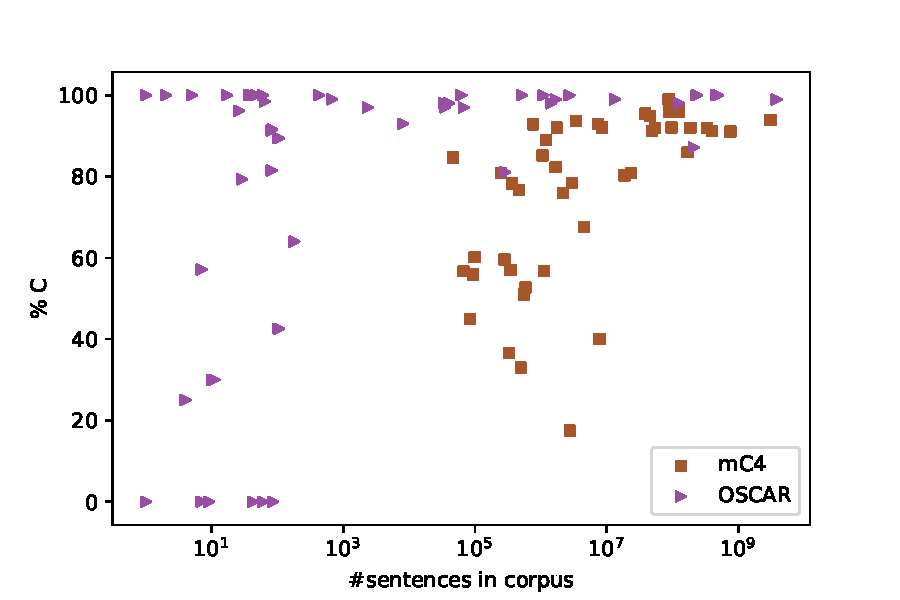
\includegraphics[width=\linewidth]{static/media/data/quality/C_mono.pdf}
        \caption{Monolingual corpora}
        \label{fig:C_mono}
    \end{subfigure}%
    \begin{subfigure}{.5\textwidth}
        \centering
        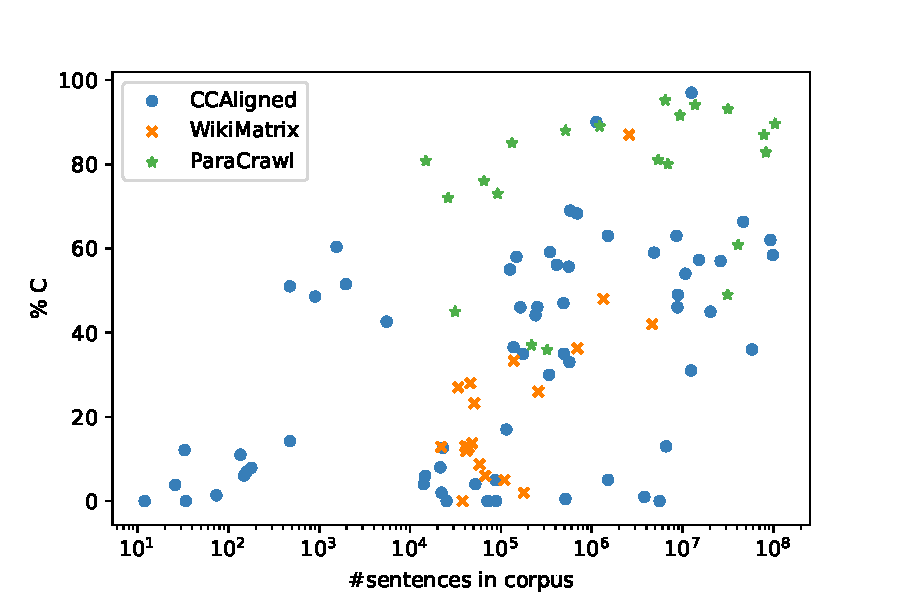
\includegraphics[width=\linewidth]{static/media/data/quality/C_para.pdf}
        \caption{Parallel corpora}
        \label{fig:C_para}
    \end{subfigure}
    \caption{Percentage of sentences labeled as correct vs. log N sentences for all audited languages.}
    \label{fig:C}
\end{figure*}

\begin{figure}[th]
    \centering
    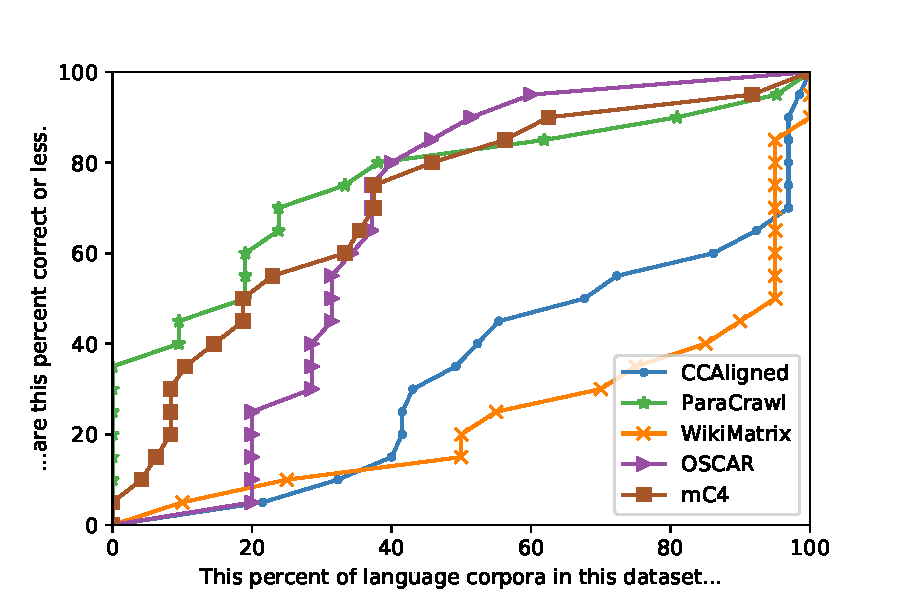
\includegraphics[width=\columnwidth]{static/media/data/quality/num_C_ratio.pdf}
    \caption{Fraction of languages in each dataset below a given quality threshold (percent correct).}% The larger the AUC, the better.}
    \label{fig:ratio_c}
\end{figure}


%In order to verify if lower-resource languages in particular have lower quality, we compare the overall rates with the mean quality of the smallest 20\% and 50\% of languages. We observe that the quality for the 20\% smallest languages is much smaller than the overall mean, especially for CCAligned with a difference of 14\% points. The amount of incorrect translations (but in the right language) is also higher for the smallest languages (32\% point for the smallest 50\%). For OSCAR, the drop in quality is not as pronounced, because it has overall lower quality. MC4 and OSCAR differ by 20\% points overall, but their quality on the smallest 20\% is comparable.
%From this comparison we conclude that \emph{the quality for the least represented languages in the multilingual mix is considerably lower, even more so when the corpus is parallel.}

\paragraph{Which languages have the lowest quality?} Across datasets we observe that the quality is particularly poor for languages that are included in the datasets in romanized script, but are more commonly written in other scripts, e.g., Urdu (\texttt{ur}), Hindi (\texttt{hi}), Arabic (\texttt{ar}). %, Chinese (\texttt{zh}), Telugu (\texttt{te}) and Bulgarian (\texttt{bg}).  
In terms of geography, the poorest quality is found for African languages (\texttt{bm}, \texttt{ff}, \texttt{kg}, \texttt{lg}, \texttt{ln}, \texttt{nso}, \texttt{om}, \texttt{sn}, \texttt{so}, \texttt{tn}, \texttt{wo}), minority languages in Europe and the Middle East that are closely related to higher-resource languages (\texttt{az-IR}, \texttt{frr}, \texttt{nap}, \texttt{szl}, \texttt{zza}), lesser spoken Chinese languages sharing a script with Mandarin (\texttt{yue}, \texttt{wuu}), and four major Austronesian languages (\texttt{bcl}, \texttt{cbk}, \texttt{jv}, \texttt{su}).
%Appendix~\ref{app:stats} contains the detailed per-language statistics for all corpora. 
% Omitted from above: mt

\paragraph{What is the incidence of offensive and pornographic content?}
Overall, the sampled sentences did not contain a large amount of offensive contents. However, there were notable amounts of pornographic content ($>10\%$) found in CCAligned for 11 languages. % not fully annotated: tl_XX, lt_LV ?

%\paragraph{Inter-annotator agreement}
\paragraph{Annotation quality}
For six audited languages from OSCAR and ten from CCAligned we measure the accuracy of the labels assigned by non-proficient speakers against the labels assigned by proficient speakers for all audited sentences. With the full 6-class taxonomy we find a mean accuracy of 0.66
%($\sigma^2 =0.02$) 
for CCAligned audits, and 0.98
%($\sigma^2 =0.002$) 
for OSCAR audits (see appendix~\ref{app:agreement} for language-specific results). With a binary taxonomy distinguishing \texttt{C} from the rest, the accuracy further increases to 0.79
%($\sigma^2=0.01$) 
for CCAligned. This provides strong evidence that good quality annotations are not limited to those proficient in a language.

\subsection{Automatic Filtering}
Given the frequency of \texttt{WL} and \texttt{NL} annotations, it might be tempting to use open-source LangID models to post-filter data on a per-sentence(-pair) level, as OSCAR does. Unfortunately, this turns out to have its own issues.

\paragraph{Sentence-level n-gram filtering}
We classify all sentence pairs of CCAligned with CLD3. By comparing its predictions to the audit labels, we evaluate its quality on the subset of annotated samples: the classifier should detect both correct languages when the pair is annotated as \texttt{C} and \texttt{X}, and should detect incorrect languages in the pair when \texttt{WL} and \texttt{NL}. On this task, the CLD3 classifier
%\footnote{\texttt{filter=0.976 Prec, 0.962 Rec, 0.969 F1.}} 
achieves an average precision of only 40.6\%. %,
%n average accuracy of 56.4\% against our annotators across all audited sentences, 
%underlining the issues with LangID on web domain data~\citep{caswell-etal-2020-language}. %Its recall for detecting those pairs with wrong language(s) is 77.8\%, and its precision 35.9\%. 

\paragraph{Transformer-based LangID filtering}
N-gram LangID models like CLD3 have known problems. However, \citet{caswell-etal-2020-language} demonstrate that semi-supervised transformer-based LangID models strongly out-perform them. We train a comparable transformer-based LangID model and apply it to our annotated CCAligned data. We find that filtering noisy corpora ($<$ 50\% correct) on LangID for both source and target leads to gains in median precision, rising from 13.8\% pre-filter to 43.9\% post-filter. However, this comes at a steep cost of 77.5\% loss in recall.
The biggest winners were Lingala, whose precision climbs from 8\% to 80\%, and Oromo, which soars from 2\% to 33\% in-language. Both of these, however, come at the cost of losing 50\% of the correct in-language sentences. The moral is that, at least at the current stage, there is no one-size-fits-all approach for sentence-level LangID.


\section{Dataset Mis-labeling}
\label{sec:codes}

% Besides general data quality issues, we found a range of problems and inconsistencies with language codes, ranging from serious mislabelings to small transgressions against standard conventions. 

%In order to use data for any practical application, it is important to have a 
Standardized and unambiguous representations of language codes are important for practical data use and exchange. The standard for unambiguous language codes used by most academic and industry applications is BCP-47~\citep{phillips-etal-2005-tags}, which would  enhance transparency and interoperability if adopted consistently. % since it allows to add subtags for scripts or regional varieties. 
%, which builds off the two-letter ISO639-2 codes and three-letter ISO639\nobreakdash-3 codes. Codes may additionally specify ISO15924 script subtags to indicate that a nonstandard script is used (e.g. \texttt{hi-Latn} for Hindi written in Latin script), ISO3166-1 country codes to indicate regional varieties (e.g. \texttt{fr-CA} for Canadian French), or extensions for private use (e.g. \texttt{ca-x-val} for Valencian Catalan). Some BCP-47 codes represent groups of languages---for instance, \texttt{kg} represents the Kongo language, and \texttt{kng}, \texttt{ldi}, \texttt{kwy}, and \texttt{yom} represent particular varieties of Kongo.

We find a variety of errors in language code usage, ranging from serious mislabelings to small transgressions against standard conventions. . For this analysis, we also include the JW300~\citep{agic-vulic-2019-jw300} dataset, a multilingual dataset crawled from \url{jw.org}. %, which was otherwise not audited in this paper. 
In summary, we find 8 nonstandard codes in CCAligned, 3 in OSCAR, 1 in mC4, 1 in WikiMatrix, and 70 in JW300, for 83 in total. This does not include the 59 codes affected by superset issues. %0 in ParaCrawl, 
Full details are given in appendix~\ref{app:jw300}.
% \subsection{Inconsistent Language Codes}

% One consistent issue is the inconsistent use of language codes. For instance,

\paragraph{Inconsistent Language Codes} One common issue is simply using nonstandard or invented codes. For example, CCAligned uses only two-letter codes, so when the BCP-47 code for a language is three letters it is either shortened (e.g. \texttt{zza} $\rightarrow$ \texttt{zz})
%, \texttt{szl}  $\rightarrow$ \texttt{sz}, \texttt{nso}  $\rightarrow$ \texttt{ns}, \texttt{ckb}  $\rightarrow$ \texttt{cb}, \texttt{ber}  $\rightarrow$ \texttt{tz} \footnote{Tamazight (BCP-47 ber) goes by various codes, so this may have been a shortening of e.g. \texttt{tzm}}) 
or invented (\texttt{shn}  $\rightarrow$ \texttt{qa})
%, \texttt{kac}  $\rightarrow$ \texttt{qd}, \texttt{ceb}  $\rightarrow$ \texttt{cx}), which can lead to 
%this can lead to confusion and limits the compatibility with other tools and resources.
Similarly, OSCAR contains data labeled as \texttt{als} (BCP-47 for Tosk Albanian) that is actually in \texttt{gsw} (Allemanic).
%\footnote{This is a result of the language code used by the Alemanic Wikipedia, and affects any corpus or tool that uses Wikipedia data without correcting for this, like FastText.} 
% \citep{joulin-etal-2017-bag, joulin-etal-2016-fasttext}.
%\footnote{\url{https://en.wikipedia.org/wiki/Alemannic_Wikipedia}
% And in JW300~\citep{agic-vulic-2019-jw300}, a multilingual dataset otherwise not audited in this paper, there are five codes ({\tt cat}, {\tt daf}, {\tt que}, {\tt nya}, {\tt run}) which use ISO693-3 instead of BCP-47 codes. Puzzlingly, in most of these cases there exist separate datasets for the equivalent ISO693-2 and 3 codes (e.g. both {\tt ny} and {\tt nya}).
22 additional language codes in JW300 have similar issues,
%mostly from mis-parsed private-use extensions, 
including 12 codes that start with \texttt{jw\_} but are not %(as they may appear)
Javanese.

% \subsection{False Language Codes}

\paragraph{False sign languages}
12\% (48/417) of JW300
%has a much stranger problem than nonstandard codes. It has the peculiar issue that a full 12\% (48/417) of the languages it claims to cover 
carry language codes for sign languages. %While it is possible to transcribe sign languages using glosses, this is not what these corpora are. 
Instead of sign language transcripts they are texts in another high resource language, mostly English or Spanish---for example, the \texttt{en-zsl} data is actually English-English parallel data (i.e. copies). %Details are in appendix table~\ref{tab:signlanguages}.


\paragraph{Mysterious supersets}
When datasets contain language codes that are supersets of other language codes, it is difficult to determine which particular language the data are in. WikiMatrix has Serbian (\texttt{sr}), Croatian (\texttt{hr}), Bosnian (\texttt{bs}), and Serbo-Croatian (\texttt{sh})---their superset. %\footnote{https://iso639-3.sil.org/code/hbs} 
%. And while there may be some debate whether \texttt{bs},  \texttt{hr},  \texttt{cnr},  and \texttt{sr} are different languages, \texttt{sh} (\texttt{hbs}) is by definition a superset of all of them.\footnote{https://iso639-3.sil.org/code/hbs} 
%The issue of codes that are supersets of others is common enough to include a small table dedicated to it, which we have done with appendix table~\ref{tab:supersets}. 
In some cases this may not be an issue, as with Arabic, where \texttt{ar} conventionally refers to Modern Standard Arabic, even though the code technically encompasses all dialects.
%, or where \texttt{no} typically refers to Norwegian Bokm\r{a}l (\texttt{nb}), though it technically is the superset of \texttt{nb} and \texttt{nn}. 
But in many cases, the nature of the data in the superset code remains a mystery.
% requiring detective work.


\paragraph{Deprecated codes} Finally, there are several deprecated codes that are used: \texttt{sh} in Wikimatrix, \texttt{iw} in mC4, \texttt{sh} and \texttt{eml} in Oscar, and \texttt{daf} in JW300.

% Maybe this is also out of the scope
% TODO the case of simple English in Wikipedia, as well as other languages with well known quality problems in Wikipedia: Buryat, Scots , Waray (bot), Swedish (bot), Cebuano (bot), ...

% a discussion on the issues of dialects might fit better in a paper focused on general problems of multilingual NLP, so maybe we can cut it from here to keepo the story more focused
% Stella: Makes sense to me, especially as length is challenging. I might try to work a sentence about this into the intro, but I'm planning on not writing a paragraph on this.
% TODO Stella: Languages are dialects with an army and a navy: Chinese, BCS, Arabic, Hindi/Urdu/Hindustani, Corsican/Italian/Sicilian

% doesn't ad enough; let's cut 
% Furthermore, language that have little standardized form, barely occur in writing or subsume a lot of diverse dialects, like for example Wu Chinese, have little hope of being correctly classified and adequately captured by automatic crawls, so their quality is expectedly low. 

\section{Risks of Low-Quality Data}\label{sec:risk}
% \section{Risks of Multilingual Data Releases with Low Quality}\label{sec:risk}

%Although releasing a dataset with low or no in-language content may seem innocuous enough, 
%There are several potentially harmful consequences of data releases without sufficient quality checks (or under false labels) that we would like to highlight.

\paragraph{Low quality in downstream applications}
Text corpora today are building blocks for many downstream NLP applications like question answering and text summarization---for instance, a common approach is to first train translation models on such data and then automatically translate training data for downstream models~\citep{conneau-etal-2018-xnli}. If the data used for the original systems is flawed, derived technology may fail for those languages far down the line without knowing the causes.
% The human inspection and auditing of e.g. trained vector representations to detect possible risks and misrepresentations of a subset of languages is arguably harder than manually inspecting a few samples as we did in this work.
% As our analysis has shown, low-resource languages are disproportionately affected by such problems in automatic data curation pipelines.

% \textsc{translate-train} and \textsc{translate-test} paradigms \citep{conneau-etal-2018-xnli}

\paragraph{Representation washing}
Since there are datasets which contain many low-resource languages, the community may feel a sense of progress and growing equity, despite the actual quality of the resources for these languages. %However, models often still perform poorly on NLP tasks for these languages
%Because there appear to be datasets for low-resource languages, the community may collectively feel as though progress is being made in these areas. 
Similarly, if low-quality datasets are used as benchmarks they may exaggerate model performance, making low-resource NLP appear more solved than it is---or conversely, if models perform poorly when trained with such data, it may be wrongly assumed that the task of learning models for these languages is harder than it actually is or infeasible given current resources. These effects could result in productive effort being redirected away from these tasks and languages.
%The result can be that productive effort will be directed away from these fields.

\paragraph{Trust in incorrect ``facts''} % and trust} %, algorithmic trust and automation bias}
We found many instances of parallel-looking sentences that are actually not semantically similar (appendix table~\ref{tab:not_actually_parallel}). They can cause models to produce plausible ``translations" that are factually wrong, but users may still trust them (\textit{algorithmic trust}) without verifying the information. %This is relevant for \textit{algorithmic trust}, when users increasingly trust the outputs of computers and ``algorithms" without verifying the information. 
Similarly, \textit{automation bias} \citep{skitka-etal-1999-does},
%from social psychology which refers to the bias of 
referring to humans favoring decisions made by automated systems over decisions made by humans, might amplify the issues of inaccurate translations caused by misaligned sentences.
%One variant of this issue that occurs frequently in some datasets is pornographic content.
%, which in the majority of the cases we observed were parts of misaligned sentence pairs. 
%Another effect is that models trained on misaligned pornographic content may hallucinate such content, which may be disturbing to users.


\section{Future Work}
There are a variety of ways to improve both the ease and accuracy of human evaluation, as well a few classes of issues we ignored in this paper, like close dialects. We present a slightly improved suggested rubric in appendix~\ref{app:improved}.

Ideally there can be a standard suite of automatic metrics for datasets, but more study is necessary to determine what the appropriate metrics would be. One important area missing from our analyses however is the estimated portion of a dataset which has been generated by MT,  LM systems, or bots/templates. %A prominent example is the Lsjbot\footnote{\url{https://en.wikipedia.org/wiki/Lsjbot}} which is responsible for creating 80-90\% of content for Swedish, Cebuano and Waray Wikipedia. 
The information captured in machine-generated content might still be useful for modeling, but might falsely overrepresent typical generation patterns and introduce linguistic errors or unnatural artifacts.
% Malagasy wiktionary audit: https://meta.wikimedia.org/wiki/Requests_for_comment/Large-scale_errors_at_Malagasy_Wiktionary
%https://www.vice.com/en/article/4agamm/the-worlds-second-largest-wikipedia-is-written-almost-entirely-by-one-bot

% Finally, similar studies to this in future would do well ton work more on calibrating human raters, to ensure consistent use of error categories.

% An issue that arises with the progress in building technology for some of the languages is the retrieval of machine-generated output as in-language data. This is prominent for mid- to high-resource languages for which translation systems have reached sufficient quality for website translation, as we observed for example a significant amount of translations for Ukrainian. Non-native speakers might not have noticed them during annotations, so the problem might be even larger than we might estimate now. We leave a systematic investigation to future work. A more unexpected artifact is the retrieval of published BPE vocabularies for a range of low-resource languages, such as Sundanese.\footnote{\url{https://nlp.h-its.org/bpemb/su/su.wiki.bpe.vs100000.vocab}}

\section{Conclusion \& Recommendations}\label{sec:recommendation}

Of the five multilingual corpora evaluated, we consistently found severe issues with quality, especially in the lower-resource languages. We rated samples of 205 languages, and found that 87 of them had under 50\% usable data, with a full 15 languages at 0\% in-language. We furthermore found consistent issues with mislabeled data and nonstandard language codes, particularly in the JW300 dataset, and identified 83 affected corpora, at least 48 of which were entirely spurious (Section \ref{sec:codes}). While there might have been anecdotal evidence of insufficient quality for some of the datasets, the majority of these quality issues had not been reported, nor been investigated in depth. These issues might go unnoticed for languages that are not represented in the evaluation of the crawling methods, and cause harm in downstream applications.
% In addition to quality issues we found a wide range of issues with language codes, particularly in JW300 and CCAligned, including mis-labeled data, invented codes, deprecated codes, and superset relations between language codes. %with a particular focus on low-resource languages, which are generally under-evaluated in NLP.

We therefore strongly recommend looking at samples of any dataset before using it or releasing it to the public. As we have shown, one does not need to be proficient in a language to see when there are serious quality issues, and a quick scan of 100 (or fewer!) sentences can be sufficient to detect major problems. Moreover, going through and annotating a small sample of data can bring useful insights about new ways to filter or use it.

If data quality issues are found, a wide variety of techniques can be explored, like filtering on length-ratio, LangID, TF-IDF wordlists \cite{caswell-etal-2020-language} or dictionaries~\citep{kamholz-etal-2014-panlex}; to neural approaches like LM scoring \cite{axelrod-etal-2011-domain,moore-lewis-2010-intelligent,wang-etal-2018-denoising}. Unfortunately, none of these provides a quick and easy fix, especially for low-resource languages -- data cleaning is no trivial task!

Noisy datasets are however by no means useless, at least if they contain some usable content. Therefore an alternative to filtering can be documentation~\citep{bender-etal-2021-on}. This can take the form of a per-language quality score and notes about known issues,
% ({ \it``language xx has high percentage non-linguistic content'' } etc.), 
a datasheet \citep{gebru-etal-2018-datasheets} or nutrition label \citep{holland-etal-2018-the}. However, we suggest researchers not release corpora with near-zero in-language content, as this may give the mistaken impression of usable resources.
%even where that is not actually the case.

Finally, we encourage the community to continue conducting evaluations and audits of public datasets -- similar to system comparison papers.
%-- which would help anyone interested in using these datasets for practical purposes.

% \begin{itemize}
%     \item \textbf{LangID Filtering:} As we have seen in Section \ref{sec:audit-res}, wrong-language is a very large class of errors. Per-sentence LangID filtering is a fast and straightforward way to alleviate this, but behaves differently on different languages and often has a high recall cost. As explored in \citet{caswell-etal-2020-language}, LangID models suffer from a variety of pathologies for long-tail languages, and datasets like OSCAR that apply per-sentence n-gram LangID still have wrong-language issues. However, datasets that apply no such filtering, like sentence-level CCAligned, seem to have a much higher proportion of wrong-language. In sum, although there is much headroom, there is also much work that needs to be done.
%     \item \textbf{Nonlinguistic Content Filtering:} LangID filtering will ideally help with this, but this is also not an easy task in general. However, a quick glance through one's data will often reveal particular classes of non-linguistic noise (like URLs, JavaScript, highly repeated characters and {\tt U+FFFD REPLACEMENT CHARACTER}s) that are easy to remove.
%     \item \textbf{Lexicon and Dictionary filtering} For higher linguistic precision, one can filter monolingual data with lexicons \cite{caswell-etal-2020-language} or parallel dictionaries with word-to-word dictionaries~\citep{kamholz-etal-2014-panlex}, and accept sentences/sentence pairs that meet some minimum threshold.
%     A similar approach can be used to filter out pornographic content, although word matching with existing lists such as the one used to create the Switch-C training corpus\footnote{https://github.com/LDNOOBW/List-of-Dirty-Naughty-Obscene-and-Otherwise-Bad-Words/blob/master/en} has been found to also aggressively filter out legitimate content on sexual health and education and LGBTQ advocacy, which can be a source of representational harm \cite{hovy-spruit-2016-social}.
%     In the datasets observed in this paper, it seemed as though a url-based exclusion approach could be more effective; and alternatively to filtering, the data can be let as-is with a disclaimer as in~\citet{gao-etal-2020-the}. 
%     \item \textbf{Fancier approaches:} There is a rich literature on neural filtering approaches. These are certainly very effective, though will likely have to be tuned for low-resource languages. However, we want to stress that much simpler approaches will get a person most of the way to a cleaner dataset.
%     \item \textbf{Consulting native speakers:} Although this is the gold standard, it will unfortunately not be feasible for every language in a large dataset, or for researchers without access to volunteers or crowdworkers in these languages; and, as outlined above, the majority of checking and filtering can be done by non-native speakers. Nonetheless, researchers wishing to provide high-quality data that can be trusted for high-stakes applications will benefit from consulting speakers of the languages they hope to include in their datasets.
%     \item \textbf{Non-English pivot:} Replacing English with another high-resource language which historically co-exists with a low-resource language with a community of bilingual speakers, e.g. crawling a French-Breton corpus would have been arguably a more successful endeavour than English-Breton, and the same may be true for Spanish-Basque vs. English-Basque.


%     TODO: discuss that we selected English-paired subsets, non-English centric MT: https://arxiv.org/abs/2010.11125 https://arxiv.org/abs/2010.10239, https://www.statmt.org/wmt20/pdf/2020.wmt-1.64.pdf
% \end{itemize}

%\section*{Acknowledgements}
%We would like to thank the AfricaNLP and Google reviewers who have helped us shape this paper. Furthermore, we are grateful for Ahmed El-Kishky's support and help with CCAligned and WikiMatrix size statistics.



\section{Details on Language Code Issues}
\label{app:jw300}

Section \ref{sec:codes} describes a variety of issues surrounding language codes that are unclear or incorrect. This section provides more details, focusing on the JW300 dataset.

In table \ref{tab:supersets} we provide a complete table of the datasets where one code is defined as a superset of the other by the ISO standard, and in table \ref{tab:signlanguages} we provide a complete list of the language codes in JW300 which purport to be sign language but are actually unrelated high-resource languages.

Special attention needs to be given to the JW300 dataset, which, in addition to the sign languages and superset code issues, has a variety of other peculiarities. These problems seem to originate in the codes used by jw.org\footnote{The jw.org website seems to use correct BCP-47 extensions now, however, and entering a code such as ``jw\_dmr" redirects to ``naq\_x\_dmr" }, which were apparently not checked in the creation of the JW300 dataset. An overview is provided in Table \ref{tab:jw300nonbcp}, and the following paragraphs give specifics.

Twelve languages in JW300 have codes starting in \texttt{jw\_}, suggesting they are varieties of Javanese (ISO639-1 \texttt{jw}), but are instead attempts to represent language dialects for which there are not BCP-47 codes. These codes seem to have been updated in jw.org to appropriate BCP-47 private-use extensions in the form \texttt{<supercode>\_x\_<tag>}, which are provided in Table \ref{tab:jw300nonbcp}.

In addition to the \texttt{jw\_} tags, there are two other mis-used private subtags: \texttt{hy\_arevmda}, which in addition to lacking the mandatory \texttt{\_x\_} appears to represent standard Western Armenian (\texttt{hyw}); and \texttt{rmy\_AR}, which, rather than being Romany from Argentina, is Kalderash Romany.

There are also a few anomalies where private use extensions should have been used but other methods were found to convey the distinctions. Three codes appear in addition to equivalent ISO codes, making it unclear which languages they are. Two of these are equivalencies between  ISO639-2 and  ISO639-3 (\texttt{nya} and \texttt{ny} are both Chichewa, \texttt{qu} and \texttt{que} are both Quechua). and one is a script equivalency (\texttt{kmr} and \texttt{kmr\_latn} are both in Latin script). In these three cases the two codes do represent different languages --- so a private use extension would have been appropriate.

Finally, there is the more minor issue that three languages use the ISO639-3 code instead of the ISO639-2 code, and therefore are not BCP-47.


In addition to the JW300-specific tables, Table \ref{tab:misc_codes} summarizes misc errors in CCAligned and OSCAR that were detailed in Section \ref{sec:codes}.

\begin{table*}[t]
    \centering
    \begin{tabular}{lll}
        \toprule
        Dataset    & supercode & subcode(s)                      \\
        \hdashline
        JW300      & kg        & kwy                             \\
        JW300      & mg        & tdx                             \\
        JW300      & qu        & que,qug,qus,quw,quy,quz,qvi,qvz \\
        JW300      & sw        & swc                             \\
        \hdashline
        OSCAR      & ar        & arz                             \\
        OSCAR      & az        & azb                             \\
        OSCAR      & sh        & bs,hr,sr                        \\
        OSCAR      & ku        & ckb                             \\
        OSCAR      & ms        & id,min                          \\
        OSCAR      & no        & nn                              \\
        OSCAR      & sq        & als$^{*}$                       \\
        OSCAR      & zh        & yue,wuu                         \\
        %  \hdashline
        % Tatoeba & ar & acm,afb,ajp,apc,arq,ary,arz,ayl \\
        % Tatoeba & ber & kab \\
        % Tatoeba & et & vro \\
        % Tatoeba & ku & ckb,kmr,sdh \\
        % Tatoeba & lv & ltg \\
        % Tatoeba & sq & aln \\
        \hdashline
        Wikimatrix & ar        & arz                             \\
        Wikimatrix & sh        & bs,hr,sr                        \\
        Wikimatrix & zh        & wuu                             \\
        \bottomrule
    \end{tabular}
    \caption{Situations where two language codes are represented, but one is a superset of another by the ISO standard, leading to unclarity about the data in the supercode dataset. $^{*}$The \texttt{als} dataset is actually in \texttt{gsw}.}
    \label{tab:supersets}
\end{table*}



\begin{table*}[t]
    \centering
    \begin{tabular}{ll}
        \toprule
        Actual language & Code in JW300                       \\
        \hdashline
        cs              & cse                                 \\
        de              & gsg                                 \\
        el              & gss                                 \\
        en              & ase,asf,bfi,ins,psp,sfs,zib,zsl     \\
        es              & aed,bvl,csf,csg,csn,csr,ecs,esn,    \\
                        & gsm,hds,lsp,mfs,ncs,prl,pys,ssp,vsl \\
        fi              & fse                                 \\
        fr              & fcs,fsl                             \\
        hu              & hsh                                 \\
        id              & inl                                 \\
        it              & ise                                 \\
        ja              & jsl                                 \\
        ko              & kvk                                 \\
        pl              & pso                                 \\
        pt              & bzs,mzy,psr,sgn\_AO                 \\
        ro              & rms                                 \\
        ru              & rsl                                 \\
        sk              & svk                                 \\
        sq              & sql                                 \\
        st              & jw\_ssa                             \\
        zh              & csl,tss                             \\
        \bottomrule
    \end{tabular}
    \caption{There are 48 languages in the JW300 corpus with language codes that correspond to sign languages, but in reality are unrelated high-resource languages (usually the most spoken language in the country of origin of the sign language). This table shows the actual language of the data corresponding to each sign language code.} %  For instance, the \texttt{ase-en} parallel data is actually \texttt{en-en} parallel data (copied source and target).
    \label{tab:signlanguages}
\end{table*}



\begin{table*}[th]
    \centering
    \begin{tabular}{lll}
        \toprule
        \textbf{Code in JW300} & \textbf{BCP-47 code} & \textbf{Actual Language Name} \\
        \multicolumn{3}{c}{}                                                          \\
        \multicolumn{3}{c}{\textbf{Incorrect private-use extensions}}                 \\
        \hdashline
        hy\_arevmda            & hyw                  & Western Armenian              \\
        jw\_dgr                & os\_x\_dgr           & Digor Ossetian                \\
        jw\_dmr                & naq\_x\_dmr          & Damara Khoekhoe               \\
        jw\_ibi                & yom\_x\_ibi          & Ibinda Kongo                  \\
        jw\_paa                & pap\_x\_paa          & Papiamento (Aruba)            \\
        jw\_qcs                & qxl                  & Salasaca Highland Kichwa      \\
        jw\_rmg                & rmn\_x\_rmg          & Greek Romani (South)          \\
        jw\_rmv                & rmy\_x\_rmv          & Vlax Romani, Russia           \\
        jw\_spl                & nso\_x\_spl          & Sepulana                      \\
        jw\_ssa                & st\_ZA               & Sesotho (South Africa)        \\
        jw\_tpo                & pt\_PT               & Portuguese (Portugal)         \\
        jw\_vlc                & ca\_x\_vlc           & Catalan (Valencia)            \\
        jw\_vz                 & skg\_x\_vz           & Vezo Malagasy                 \\
        rmy\_AR                & rmy\_x\_?            & Kalderash                     \\

        \multicolumn{3}{c}{}                                                          \\
        \multicolumn{3}{c}{\textbf{Equivalent codes used in place of extensions}}     \\
        \hdashline
        kmr\_latn              & kmr\_x\_rdu          & Kurmanji (Caucasus)           \\
        nya                    & ny\_x\_?             & Chinyanja (Zambia)            \\
        que                    & qu\_x\_?             & Quechua (Ancash)              \\

        \multicolumn{3}{c}{}                                                          \\
        \multicolumn{3}{c}{\textbf{Deprecated codes}}                                 \\
        \hdashline
        daf                    & dnj/lda              & Dan                           \\
        % sgn\_AO & 	pt & 	Portuguese \\ 

        \multicolumn{3}{c}{}                                                          \\
        \multicolumn{3}{c}{\textbf{ISO-693-3 used in place of ISO-693-2}}             \\
        \hdashline
        cat                    & ca                   & Catalan                       \\
        gug                    & gn                   & Guarani                       \\
        run                    & rn                   & Kirundi                       \\
        tso\_MZ                & ts\_MZ               & Changana (Mozambique)         \\
        \bottomrule
    \end{tabular}
    \caption{Language code issues in the JW300 datasets for 22 language varieties not covered by Tables \ref{tab:supersets} and \ref{tab:signlanguages}. Twelve languages have codes starting in \texttt{jw\_}, suggesting they are varieties of Javanese, but are instead mis-parsed private-use extensions. Three codes appear in addition to equivalent ISO codes, making it unclear which languages they are. One language uses a deprecated ISO code. Four languages use the ISO639-3 code instead of the ISO639-2 code, and therefore are not BCP-47. (Note: in this table, private use extensions are given as they appear in jw.org, and specified as `?' if they are absent from jw.org.)}
    \label{tab:jw300nonbcp}
\end{table*}



\section{Complete Error Taxonomy and Instructions}

In addition to the table given in table \ref{tab:examples}, raters were provided with the following verbal notes on the error codes
\begin{itemize}
    \item \textbf{\texttt{CC}: Correct translation, natural sentence:} It's OK if it's a sentence fragment instead of a whole sentence, as long as it is not too short (about 5 words or greater). The translation does not have to be perfect.
    \item \textbf{\texttt{\texttt{CS}}: Correct Translation, but single word or short phrase:} Also includes highly repeated short phrases, like ``the cat the cat the cat the cat the cat ..."
    \item \textbf{\texttt{CB}: Correct translation, but boilerplate: } This can be auto-generated or formulaic content, or content that one deems ``technically correct but generally not very useful to NLP models". Unfortunately, it's often not clear what should be counted as boilerplate...do your best.
    \item \textbf{\texttt{X}: Incorrect translation} [for parallel sentences] both source and target are in the correct language, but they are not adequate translations.
    \item \textbf{\texttt{WL}: Wrong language} For short sentences, especially with proper nouns, there is often a fine line between ``Wrong language" and ``Not language". Do your best.
    \item \textbf{\texttt{NL}: Not language} At least one of source and target are not linguistic content. Any sentence consisting only of a proper noun (e.g. ``Tyrone Ping") should be marked as \texttt{NL}.
    \item \textbf{\texttt{U}: Unknown} for sentences that need verification by a native speaker. This is an auxiliary label that is resolved in most cases.
\end{itemize}

%Additionally, we provide a few examples of incorrect translations (\texttt{X}) in table \ref{tab:not_actually_parallel} demonstrating common patterns we saw, where sentences have superficial similarity but represent different facts, spelling potential danger for models trained on them.

Finally, for future work please consider using the aspirational error taxonomy in appendix \ref{app:improved}, rather than the one presented above.

\begin{table*}[!htbp]
    \centering
    \resizebox{\textwidth}{!}{%

        \begin{tabular}{lcccccccccccc}
            \toprule
                           & \texttt{es\_XX} & \texttt{bm\_ML} & \texttt{yo\_NG} & \texttt{tr\_TR} & \texttt{ku\_TR} & \texttt{zh\_CN} & \texttt{af\_ZA} & \texttt{jv\_ID} & \texttt{zh\_TW} & \texttt{it\_IT} & \textbf{mean} \\
            \midrule
            \textbf{Acc-6} & 0.58            & 0.73            & 0.41            & 0.45            & 0.43            & 0.55            & 0.65            & 0.55            & 0.46            & 0.55            & 0.66          \\
            \textbf{Acc-4} & 0.77            & 0.73            & 0.60            & 0.55            & 0.56            & 0.72            & 0.72            & 0.57            & 0.58            & 0.66            & 0.72          \\
            \textbf{Acc-2} & 0.91            & 0.96            & 0.72            & 0.64            & 0.71            & 0.79            & 0.77            & 0.92            & 0.81            & 0.69            & 0.79          \\
            \bottomrule
        \end{tabular}%
    }
    \caption{Rater evaluation for a subset of audits from \textbf{CCAligned} (translated from English) measured by the accuracy (Acc-$n$) of labels assigned by non-proficient speaker against those assigned by proficient speakers. $n$ indicates the granularity of the classes.  For $n=6$ all classes of the taxonomy were distinguished, for $n=4$ the \texttt{C} subclasses were combined, and for $n=2$ it is binary decision between \texttt{C} and the rest of the error classes.}
    \label{tab:agreement_ccaligned}
\end{table*}

\clearpage

\begin{table}[!htbp]
    \centering
        \begin{tabular}{lccccccccc}
            \toprule
                           & \texttt{tyv} & \texttt{rm} & \texttt{bar} & \texttt{eml} & \texttt{zh} & \texttt{la} & \textbf{mean} \\
            \midrule
            \textbf{Acc-6} & 1.0          & 0.98        & 1.0          & 1.0          & 0.86        & 1.0         & 0.98          \\
            \textbf{Acc-4} & 1.0          & 1.0         & 1.0          & 1.0          & 0.87        & 1.0         & 0.98          \\
            \textbf{Acc-2} & 1.0          & 1.0         & 1.0          & 1.0          & 0.87        & 1.0         & 0.98          \\
            \bottomrule
        \end{tabular}%
    \caption{Rater evaluation for a subset of audits from \textbf{OSCAR} measured by the accuracy (Acc-$n$) of labels assigned by non-proficient speaker against those assigned by proficient speakers.  $n$ indicates the granularity of the classes. For $n=6$ all classes of the taxonomy were distinguished, for $n=4$ the \texttt{C} subclasses were combined, and for $n=2$ it is binary decision between \texttt{C} and the rest of the error classes.}
    \label{tab:agreement_oscar}
\end{table}


\begin{table}[!ht]
    \small
    \centering
    \begin{tabular}{lll}
        \toprule
        corpus     & code in corpus & correct code \\
        \hline
        CCAligned  & zz             & zza          \\
        CCAligned  & sz             & szl          \\
        CCAligned  & ns             & nso          \\
        CCAligned  & cb             & ckb          \\
        CCAligned  & tz             & ber          \\
        CCAligned  & qa             & shn          \\
        CCAligned  & qd             & kac          \\
        CCAligned  & cx             & ceb          \\
        mC4        & iw             & he           \\
        OSCAR      & eml            & egl          \\
        OSCAR      & als            & gsw          \\
        OSCAR      & sh             & hbs          \\
        Wikimatrix & sh             & hbs          \\
        \bottomrule
    \end{tabular}
    \caption{Miscellaneous errors in language codes not in other tables (mentioned in the text in Section \ref{sec:codes}).}
    \label{tab:misc_codes}
\end{table}


\section{Non-proficient Rater Evaluation}\label{app:agreement}

Tables~\ref{tab:agreement_ccaligned} and~\ref{tab:agreement_oscar} show the detailed rating accuracy scores for all selected languages for several levels of annotation granularity. We can see that for the CCAligned data, reducing the labels to a binary scale naturally increases the accuracy (except for \texttt{tr\_TR}), so a binary interpretation (``correct" sentence vs. error) is the most reliable. For monolingual data, the accuracy appears exceptionally high since the \texttt{bar} and \texttt{tyv} corpora contain $<100$ sentences each (4 and 25, respectively).


\begin{table}[!ht]
    \small
    \centering
    \begin{tabular}{ll}
        \toprule

        \texttt{en}  & The prime minister of the \textbf{UK} is \textbf{Boris Johnson}.     \\
        \texttt{nl}  & De minister-president van \textbf{Nederland} is \textbf{Mark Rutte}. \\
        \hdashline
        % \texttt{en} &Sunglasses \\
        % \texttt{ig}	&ah\d{i}a Nyocha \\
        % \hdashline
        \texttt{en}  & \textbf{24 March} 2018                                               \\
        \texttt{pt}  & \textbf{14 Novembro} 2018                                            \\
        \hdashline
        % \texttt{en} &The current local time in \textbf{Sarasota} is \textbf{89} minutes ahead of apparent solar time. \\
        % \texttt{nn}	&Den lokale tiden i \textbf{Miami} er \textbf{86} minutt f\o{o}re sann soltid. \\
        \texttt{en}  & The current local time in \textbf{Sarasota} is \textbf{89} minutes.  \\
        \texttt{nn}  & Den lokale tiden i \textbf{Miami} er \textbf{86} minutt.             \\
        \hdashline
        \texttt{en}  & In \textbf{1932} the highway was extended \textbf{north to LA}.      \\
        \texttt{bar} & \textbf{1938} is de Autobahn bei \textbf{Inglstod} fertig gstellt.   \\
        % \hdashline
        % \textit{en:} He was engaged to the lawyer and actor João Lima Junior, with whom he dated from 2004 to 2006. \\
        % \textit{nds:} Ze woont in de tussentied samen met zanger en liedtiesschriever Johannes Oerding met wie ze sinds 2009 ook samen op de bühne stiet.\\
        \bottomrule
    \end{tabular}
    \caption{Examples of ``parallel" data where the translation has a different meaning than the source, but the form looks the same. Such data may encourage hallucinations of fake ``facts".}
    \label{tab:not_actually_parallel}
\end{table}

\section{Not-So-Parallel Data}
Table~\ref{tab:not_actually_parallel} contains a list of examples from the audited datasets that were misaligned  (\texttt{X}). These examples in particular illustrate that structurally similar sentences can easily describe very different facts. Translation models trained on such examples might hallucinate such fact-altering translations.


\section{Quality vs Size}\label{app:plots}
To understand the relation between the amount of data available for each language in each corpus and the quality as estimated by our audit, we plot the ratio of \texttt{X}, \texttt{NL} and \texttt{WL} labels against the number of sentences in figures~\ref{fig:c_app},~\ref{fig:x},~\ref{fig:nl},~\ref{fig:wl}.






\section{Methodological Notes}\label{app:strategies}

A surprising amount of work can be done without being an expert in the languages involved. The easiest approach is simply to search the internet for the sentence, which usually results in finding the exact page the sentence came from, which in turn frequently contains clues like language codes in the URL, or a headline like \textit{News in X language}, sometimes with references to a translated version of the same page. However, for the cases where this is insufficient, here are a few tips, tricks, and observations.

\subsection*{No Skills Required}
Things that do not require knowledge of the language(s) in question.

\begin{enumerate}
    \item ``Not language'' can usually be identified by anyone who can read the script, though there are tricky cases with proper nouns.
    \item Frequently, ``parallel" sentences contain different numbers in the source and target (especially autogenerated content), and are easy to disqualify
    \item Errors tend to repeat. If a word is mistranslated once, it will often be mistranslated many more times throughout a corpus, making it easy to spot
\end{enumerate}

\subsection*{Basic Research Required}
Things that do not require knowledge of the language(s) in question but can be done with basic research.
\begin{enumerate}
    \item If it's written in the wrong script it's considered wrong language. (Sometimes the writing system is indicated in the published corpus, e.g. \texttt{bg-Latn}, but usually the language has a ``default" script defined by ISO.)
    \item Some types of texts come with inherent labels or markers, such as enumerators or verse numbers.
          %For example, much of CCAligned's Odia text is Christian Bible verses, which are preceded by an identifier like ``Matt 12:37". 
    \item When all else fails, search the internet for the whole sentence or n-grams thereof! If the whole sentence can be found, frequently the language is betrayed by the webpage (the language's autonym is useful in this case).
\end{enumerate}



% \subsection{Weak Knowledge}

% Things that can be done by people with weak knowledge of the language(s) or strong knowledge of a related language.

% \begin{enumerate}
%     \item Some types of texts come with inherent labels or markers, such as enumerators or verse numbers. For example, much of CCAligned's Odia text is Christian Bible verses. 
% \end{enumerate}



\begin{figure*}[ht]
    \label{ fig7}
    \begin{minipage}[b]{0.5\linewidth}
        \centering
        \includegraphics[width=\linewidth]{static/media/data/quality/C.pdf}
        \caption{Ratio of \texttt{C} ratings vs size.}
        \label{fig:c_app}
        \vspace{4ex}
    \end{minipage}%%
    \begin{minipage}[b]{0.5\linewidth}
        \centering
        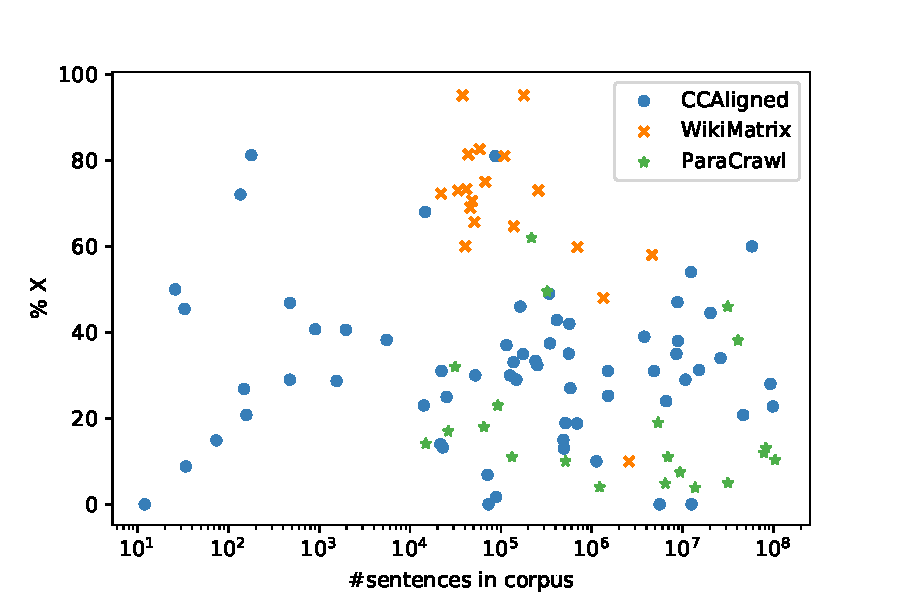
\includegraphics[width=\linewidth]{static/media/data/quality/X.pdf}
        \caption{Ratio of \texttt{X} ratings vs size.}
        \label{fig:x}
        \vspace{4ex}
    \end{minipage}
    \begin{minipage}[b]{0.5\linewidth}
        \centering
        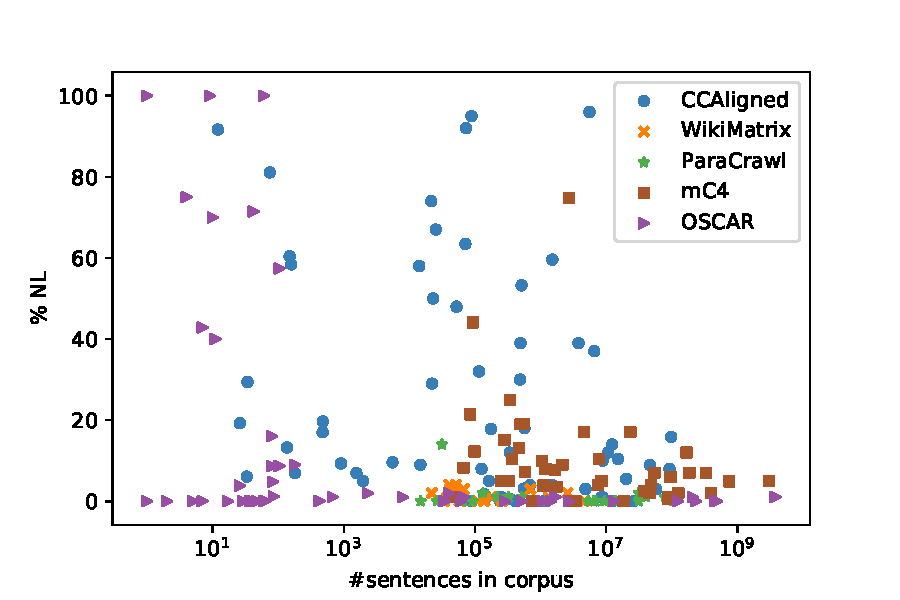
\includegraphics[width=\linewidth]{static/media/data/quality/NL.pdf}
        \caption{Ratio of \texttt{NL} ratings vs size.}
        \label{fig:nl}
        \vspace{4ex}
    \end{minipage}%% 
    \begin{minipage}[b]{0.5\linewidth}
        \centering
        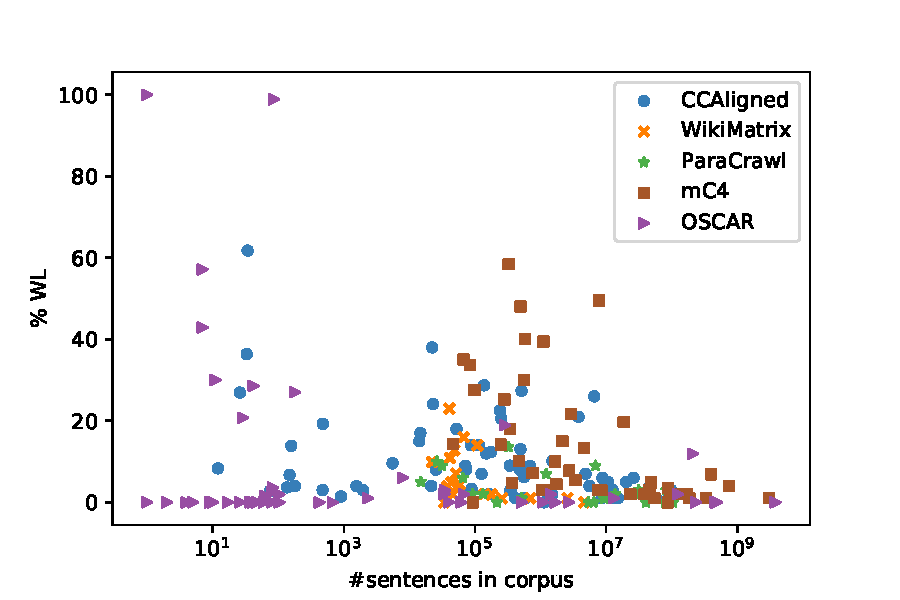
\includegraphics[width=\linewidth]{static/media/data/quality/WL.pdf}
        \caption{Ratio of \texttt{WL} ratings vs size.}
        \label{fig:wl}
        \vspace{4ex}
    \end{minipage}
\end{figure*}


\section{Aspirational Error Taxonomy}
\label{app:improved}

Although the error taxonomy used in this paper did the job, there are a variety of ways to improve both the ease and accuracy of human evaluation, as well as the ease of automatically detecting issues and fixing them. With respect to improved annotations, the error taxonomy presented in this paper lacks at least one significant category of error, namely ``correct/in-language but unnatural".  Similarly, the definition of ``correct-short" and ``correct-boilerplate" were not understood equally by all annotators, leading us to collapse the categories into one for most analyses. Similarly, a concept like ``correct-short" has potential issues for agglutinative languages like Turkish. Finally, it was unclear what to do with related dialects, e.g. when a sentence is ``almost correct but wrong dialect" or when it is unclear which dialect a sentence belongs to.

Therefore, we present here a slightly modified version which we hope is both more explicit and finer-grained. The main changes are 1) replacing ``CB" and ``CS" with a catch-all for lower-quality sentences ``CL", and 2) incorporating two codes for languages with related dialects. This is also by no means a perfect rubric, and would benefit from some fine-tuning and workshopping based on the particular dataset or application in question.

\begin{itemize}
    \item \textbf{\texttt{CC}: Correct:} Natural in-language sentence. It's ok if it has a few small issues, like spelling errors or a few words from another language, or if it’s a sentence fragment of reasonable length (about 5 words or more). For translations, there may be minor mistakes in the translation.
    \item \textbf{\texttt{\texttt{CL}}: Correct Low-quality:} In-language sentence, but low-quality. This could be ungrammatical text, boilerplate, or very short fragments. For translations, this is the appropriate code for a low-quality translation.
    \item \textbf{\texttt{X}: Incorrect translation} [for parallel sentences] both source and target are in the correct language, but they are not adequate translations.
    \item \textbf{\texttt{DW}: Wrong Dialect} \textit{This code is only applicable for dialects that are closely related to other languages/dialects.} This sentence is in a related but different dialect to the language it's supposed to be in. For instance, it's supposed to be in Sa'idi Arabic but it's in Egyptian Arabic.
    \item \textbf{\texttt{DA}: Ambiguous Dialect} \textit{This code is only applicable for dialects that are closely related to other languages/dialects.} Correct but ambiguous whether it's in the correct language. For instance, many short sentences in Gulf Arabic may also be valid in MSA, and many written Cantonese sentences might also be valid in Mandarin.
    \item \textbf{\texttt{WL}: Wrong language} This sentence is not in the language it's supposed to be. For short sentences, especially with proper nouns, there is often a fine line between ``Wrong language" and ``Not language". Do your best.
    \item \textbf{\texttt{NL}: Not language} At least one of source and target are not linguistic content. Any sentence consisting only of a proper noun (e.g. ``Ibuprofin", ``Calvin Klein", or ``Washington DC") should be marked as \texttt{NL}
    \item \textbf{\texttt{U}: Unknown} for sentences that need verification by a native speaker. This is an auxiliary label that is resolved in most cases.
\end{itemize}

\textbf{Special note on Boilerplate:} ``Boilerplate" generally refers to autogenerated text found on websites. It's not always clear when a sentence is boilerplate or not. If you see a lot of similar formulaic sentences in the sample, however, that's a good sign that they are boilerplate, and you can mark them all as ``CL" ! Common types of boilerplate include sentences like ``Convert Euro to Pound", ``Online gambling games", ``Download Game of Thrones Free Torrent" and so on.


\textbf{Special note on Mixed Language:} Some samples are mixed between the right language and some other language. Some out-of-language content is fine, but a majority out-of-language content is not. We can mark the sentence ``CC" if: 1) it is majority in-language, and 2) the in-language portion is more than a short phrase. For unclear border cases you can use “CL”.


\section{Complete Tables}\label{app:stats}
Tables \ref{tab:ccaligned-full}, \ref{tab:mc4-full}, \ref{tab:oscar-full}, \ref{tab:paracrawl-full}, and \ref{tab:wikimatrix-full} give the complete annotation percentages for CCAligned, MC4, OSCAR, Paracrawl, and Wikimatrix, respectively.
